% Options for packages loaded elsewhere
\PassOptionsToPackage{unicode}{hyperref}
\PassOptionsToPackage{hyphens}{url}
%
\documentclass[
]{article}
\usepackage{amsmath,amssymb}
\usepackage{lmodern}
\usepackage{ifxetex,ifluatex}
\ifnum 0\ifxetex 1\fi\ifluatex 1\fi=0 % if pdftex
  \usepackage[T1]{fontenc}
  \usepackage[utf8]{inputenc}
  \usepackage{textcomp} % provide euro and other symbols
\else % if luatex or xetex
  \usepackage{unicode-math}
  \defaultfontfeatures{Scale=MatchLowercase}
  \defaultfontfeatures[\rmfamily]{Ligatures=TeX,Scale=1}
\fi
% Use upquote if available, for straight quotes in verbatim environments
\IfFileExists{upquote.sty}{\usepackage{upquote}}{}
\IfFileExists{microtype.sty}{% use microtype if available
  \usepackage[]{microtype}
  \UseMicrotypeSet[protrusion]{basicmath} % disable protrusion for tt fonts
}{}
\makeatletter
\@ifundefined{KOMAClassName}{% if non-KOMA class
  \IfFileExists{parskip.sty}{%
    \usepackage{parskip}
  }{% else
    \setlength{\parindent}{0pt}
    \setlength{\parskip}{6pt plus 2pt minus 1pt}}
}{% if KOMA class
  \KOMAoptions{parskip=half}}
\makeatother
\usepackage{xcolor}
\IfFileExists{xurl.sty}{\usepackage{xurl}}{} % add URL line breaks if available
\IfFileExists{bookmark.sty}{\usepackage{bookmark}}{\usepackage{hyperref}}
\hypersetup{
  pdftitle={HW4-tk2886},
  pdfauthor={Tanvir Khan},
  hidelinks,
  pdfcreator={LaTeX via pandoc}}
\urlstyle{same} % disable monospaced font for URLs
\usepackage[margin=1in]{geometry}
\usepackage{color}
\usepackage{fancyvrb}
\newcommand{\VerbBar}{|}
\newcommand{\VERB}{\Verb[commandchars=\\\{\}]}
\DefineVerbatimEnvironment{Highlighting}{Verbatim}{commandchars=\\\{\}}
% Add ',fontsize=\small' for more characters per line
\usepackage{framed}
\definecolor{shadecolor}{RGB}{248,248,248}
\newenvironment{Shaded}{\begin{snugshade}}{\end{snugshade}}
\newcommand{\AlertTok}[1]{\textcolor[rgb]{0.94,0.16,0.16}{#1}}
\newcommand{\AnnotationTok}[1]{\textcolor[rgb]{0.56,0.35,0.01}{\textbf{\textit{#1}}}}
\newcommand{\AttributeTok}[1]{\textcolor[rgb]{0.77,0.63,0.00}{#1}}
\newcommand{\BaseNTok}[1]{\textcolor[rgb]{0.00,0.00,0.81}{#1}}
\newcommand{\BuiltInTok}[1]{#1}
\newcommand{\CharTok}[1]{\textcolor[rgb]{0.31,0.60,0.02}{#1}}
\newcommand{\CommentTok}[1]{\textcolor[rgb]{0.56,0.35,0.01}{\textit{#1}}}
\newcommand{\CommentVarTok}[1]{\textcolor[rgb]{0.56,0.35,0.01}{\textbf{\textit{#1}}}}
\newcommand{\ConstantTok}[1]{\textcolor[rgb]{0.00,0.00,0.00}{#1}}
\newcommand{\ControlFlowTok}[1]{\textcolor[rgb]{0.13,0.29,0.53}{\textbf{#1}}}
\newcommand{\DataTypeTok}[1]{\textcolor[rgb]{0.13,0.29,0.53}{#1}}
\newcommand{\DecValTok}[1]{\textcolor[rgb]{0.00,0.00,0.81}{#1}}
\newcommand{\DocumentationTok}[1]{\textcolor[rgb]{0.56,0.35,0.01}{\textbf{\textit{#1}}}}
\newcommand{\ErrorTok}[1]{\textcolor[rgb]{0.64,0.00,0.00}{\textbf{#1}}}
\newcommand{\ExtensionTok}[1]{#1}
\newcommand{\FloatTok}[1]{\textcolor[rgb]{0.00,0.00,0.81}{#1}}
\newcommand{\FunctionTok}[1]{\textcolor[rgb]{0.00,0.00,0.00}{#1}}
\newcommand{\ImportTok}[1]{#1}
\newcommand{\InformationTok}[1]{\textcolor[rgb]{0.56,0.35,0.01}{\textbf{\textit{#1}}}}
\newcommand{\KeywordTok}[1]{\textcolor[rgb]{0.13,0.29,0.53}{\textbf{#1}}}
\newcommand{\NormalTok}[1]{#1}
\newcommand{\OperatorTok}[1]{\textcolor[rgb]{0.81,0.36,0.00}{\textbf{#1}}}
\newcommand{\OtherTok}[1]{\textcolor[rgb]{0.56,0.35,0.01}{#1}}
\newcommand{\PreprocessorTok}[1]{\textcolor[rgb]{0.56,0.35,0.01}{\textit{#1}}}
\newcommand{\RegionMarkerTok}[1]{#1}
\newcommand{\SpecialCharTok}[1]{\textcolor[rgb]{0.00,0.00,0.00}{#1}}
\newcommand{\SpecialStringTok}[1]{\textcolor[rgb]{0.31,0.60,0.02}{#1}}
\newcommand{\StringTok}[1]{\textcolor[rgb]{0.31,0.60,0.02}{#1}}
\newcommand{\VariableTok}[1]{\textcolor[rgb]{0.00,0.00,0.00}{#1}}
\newcommand{\VerbatimStringTok}[1]{\textcolor[rgb]{0.31,0.60,0.02}{#1}}
\newcommand{\WarningTok}[1]{\textcolor[rgb]{0.56,0.35,0.01}{\textbf{\textit{#1}}}}
\usepackage{graphicx}
\makeatletter
\def\maxwidth{\ifdim\Gin@nat@width>\linewidth\linewidth\else\Gin@nat@width\fi}
\def\maxheight{\ifdim\Gin@nat@height>\textheight\textheight\else\Gin@nat@height\fi}
\makeatother
% Scale images if necessary, so that they will not overflow the page
% margins by default, and it is still possible to overwrite the defaults
% using explicit options in \includegraphics[width, height, ...]{}
\setkeys{Gin}{width=\maxwidth,height=\maxheight,keepaspectratio}
% Set default figure placement to htbp
\makeatletter
\def\fps@figure{htbp}
\makeatother
\setlength{\emergencystretch}{3em} % prevent overfull lines
\providecommand{\tightlist}{%
  \setlength{\itemsep}{0pt}\setlength{\parskip}{0pt}}
\setcounter{secnumdepth}{-\maxdimen} % remove section numbering
\ifluatex
  \usepackage{selnolig}  % disable illegal ligatures
\fi

\title{HW4-tk2886}
\author{Tanvir Khan}
\date{}

\begin{document}
\maketitle

\hypertarget{loading-the-data}{%
\subsubsection{Loading the data}\label{loading-the-data}}

\begin{Shaded}
\begin{Highlighting}[]
\NormalTok{crash\_df }\OtherTok{\textless{}{-}} 
  \FunctionTok{read.csv}\NormalTok{(}\StringTok{"Crash.csv"}\NormalTok{)}
\end{Highlighting}
\end{Shaded}

\hypertarget{tidy-the-data}{%
\subsubsection{Tidy the data}\label{tidy-the-data}}

\begin{Shaded}
\begin{Highlighting}[]
\NormalTok{crash\_dfn }\OtherTok{\textless{}{-}}
\NormalTok{  crash\_df }\SpecialCharTok{\%\textgreater{}\%}
  \FunctionTok{pivot\_longer}\NormalTok{(}\FunctionTok{everything}\NormalTok{(), }
               \AttributeTok{names\_to =} \StringTok{"type\_of\_accidents"}\NormalTok{,}
               \AttributeTok{values\_to =} \StringTok{"Values"}\NormalTok{)}
\end{Highlighting}
\end{Shaded}

\hypertarget{problem-2a}{%
\section{Problem 2a}\label{problem-2a}}

\hypertarget{generate-descriptive-statistics-for-each-group}{%
\subsubsection{Generate Descriptive statistics for each
group}\label{generate-descriptive-statistics-for-each-group}}

\begin{Shaded}
\begin{Highlighting}[]
\NormalTok{crash\_df }\SpecialCharTok{\%\textgreater{}\%} \FunctionTok{summary}\NormalTok{()}
\end{Highlighting}
\end{Shaded}

\begin{verbatim}
##    pedestrian       bicycle          car       
##  Min.   :29.00   Min.   :28.0   Min.   :20.00  
##  1st Qu.:36.00   1st Qu.:29.5   1st Qu.:21.00  
##  Median :39.50   Median :31.5   Median :22.00  
##  Mean   :37.88   Mean   :32.5   Mean   :23.43  
##  3rd Qu.:42.00   3rd Qu.:34.5   3rd Qu.:24.50  
##  Max.   :43.00   Max.   :39.0   Max.   :31.00  
##  NA's   :2                      NA's   :3
\end{verbatim}

\begin{Shaded}
\begin{Highlighting}[]
\NormalTok{crash\_df }\SpecialCharTok{\%\textgreater{}\%} \FunctionTok{summarize\_if}\NormalTok{(is\_numeric, sd, }\AttributeTok{na.rm =}\NormalTok{ T)}
\end{Highlighting}
\end{Shaded}

\begin{verbatim}
##   pedestrian  bicycle      car
## 1    5.43632 4.062019 3.866831
\end{verbatim}

\#boxplot

\begin{Shaded}
\begin{Highlighting}[]
\FunctionTok{boxplot}\NormalTok{(Values }\SpecialCharTok{\textasciitilde{}}\NormalTok{ type\_of\_accidents, }\AttributeTok{data =}\NormalTok{ crash\_dfn,}
        \AttributeTok{main =} \StringTok{"Distribution of PTSD score for each type of crash"}\NormalTok{,}
        \AttributeTok{xlab =} \StringTok{"Types of Accident"}\NormalTok{,}
        \AttributeTok{ylab =} \StringTok{"PTSD Score"}\NormalTok{)}
\end{Highlighting}
\end{Shaded}

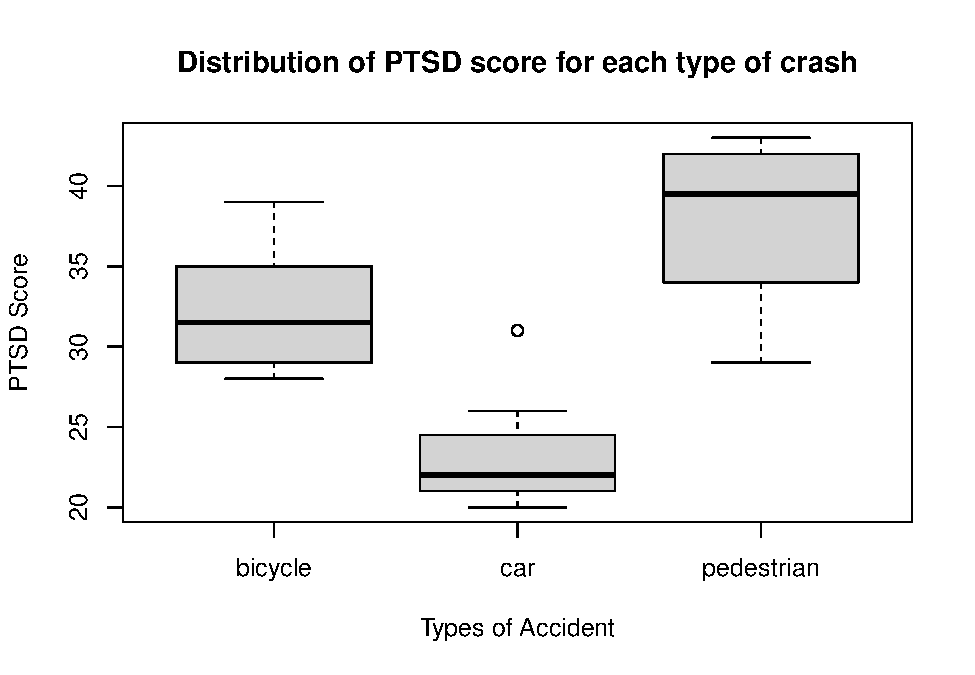
\includegraphics{HW4-tk2886-_files/figure-latex/unnamed-chunk-5-1.pdf}

\hypertarget{analysis-n-differences-observed}{%
\subsubsection{Analysis n Differences
Observed:}\label{analysis-n-differences-observed}}

In the data set that was provided, the mean of the PTSD Score for
Pedestrian Incidents is the largest among the three types of accidents.
The mean of the PTSD Score of bicycle incidents is the second highest
and the mean of the PTSD Scores for car incidents is the lowest. The
standard deviation for PTSD score for pedestrian incident is 5.44, the
standard deviation for PTSD score in bicycle incident is 4.06, and the
standard deviation for the PTSD score for car crash is 3.87. Pedestrian
has a larger standard deviation than bicycle and car. This indicates
that the PTSD score for this pedestrian incidents is more spread out
compared to the other two types if crash. When pedestrians is involved
in an incident, their PTSD in generall is more varied compared to the
other groups (bicycle and cars).

\hypertarget{problem-2b}{%
\section{Problem 2b:}\label{problem-2b}}

\begin{Shaded}
\begin{Highlighting}[]
\NormalTok{res1 }\OtherTok{=} \FunctionTok{aov}\NormalTok{(Values }\SpecialCharTok{\textasciitilde{}} \FunctionTok{factor}\NormalTok{(type\_of\_accidents), }\AttributeTok{data =}\NormalTok{ crash\_dfn)}
\FunctionTok{summary}\NormalTok{(res1)}
\end{Highlighting}
\end{Shaded}

\begin{verbatim}
##                           Df Sum Sq Mean Sq F value   Pr(>F)    
## factor(type_of_accidents)  2  790.4   395.2   19.53 1.33e-05 ***
## Residuals                 22  445.1    20.2                     
## ---
## Signif. codes:  0 '***' 0.001 '**' 0.01 '*' 0.05 '.' 0.1 ' ' 1
## 5 observations deleted due to missingness
\end{verbatim}

\begin{Shaded}
\begin{Highlighting}[]
\NormalTok{critical\_value }\OtherTok{=} \FunctionTok{qf}\NormalTok{(}\FloatTok{0.99}\NormalTok{, }\DecValTok{2}\NormalTok{, }\DecValTok{22}\NormalTok{)}
\end{Highlighting}
\end{Shaded}

\textbf{Interpretation}:

\emph{Hypothesis:} Ho: \$\mu1 \$ = \$\mu2 \$ = \$\mu3 \$

Ha: at least two means are not equal

\emph{Test-Statistics:} F-Value: 19.53

\emph{Critical Value:} Critical Value: 5.7190219

\emph{Decision Intercepted:} Our F-statistics (19.53) is bigger than our
critical value (5.72), we reject the null hypothesis. At 0.01
significance level, we reject the null hypothesis and conclude that at
least two mean PTSD score from the three type of crash groups are
different.

\hypertarget{problem-2c}{%
\section{Problem 2c:}\label{problem-2c}}

\begin{Shaded}
\begin{Highlighting}[]
\CommentTok{\# use pairwise.t.test() for Bonferroni, Holm, Benjamini{-}Hochberg}
\FunctionTok{pairwise.t.test}\NormalTok{(crash\_dfn}\SpecialCharTok{$}\NormalTok{Values, crash\_dfn}\SpecialCharTok{$}\NormalTok{type\_of\_accidents, }\AttributeTok{p.adj =} \StringTok{\textquotesingle{}bonferroni\textquotesingle{}}\NormalTok{)}
\end{Highlighting}
\end{Shaded}

\begin{verbatim}
## 
##  Pairwise comparisons using t tests with pooled SD 
## 
## data:  crash_dfn$Values and crash_dfn$type_of_accidents 
## 
##            bicycle car    
## car        0.0014  -      
## pedestrian 0.0586  9.1e-06
## 
## P value adjustment method: bonferroni
\end{verbatim}

\begin{Shaded}
\begin{Highlighting}[]
\CommentTok{\# use Tukey}
\NormalTok{Tukey\_comp }\OtherTok{=} \FunctionTok{TukeyHSD}\NormalTok{(res1)}
\NormalTok{Tukey\_comp}
\end{Highlighting}
\end{Shaded}

\begin{verbatim}
##   Tukey multiple comparisons of means
##     95% family-wise confidence level
## 
## Fit: aov(formula = Values ~ factor(type_of_accidents), data = crash_dfn)
## 
## $`factor(type_of_accidents)`
##                         diff          lwr       upr     p adj
## car-bicycle        -9.071429 -14.63967214 -3.503185 0.0013441
## pedestrian-bicycle  5.375000   0.01537946 10.734621 0.0492580
## pedestrian-car     14.446429   8.59860314 20.294254 0.0000088
\end{verbatim}

\begin{Shaded}
\begin{Highlighting}[]
\FunctionTok{plot}\NormalTok{(Tukey\_comp)}
\end{Highlighting}
\end{Shaded}

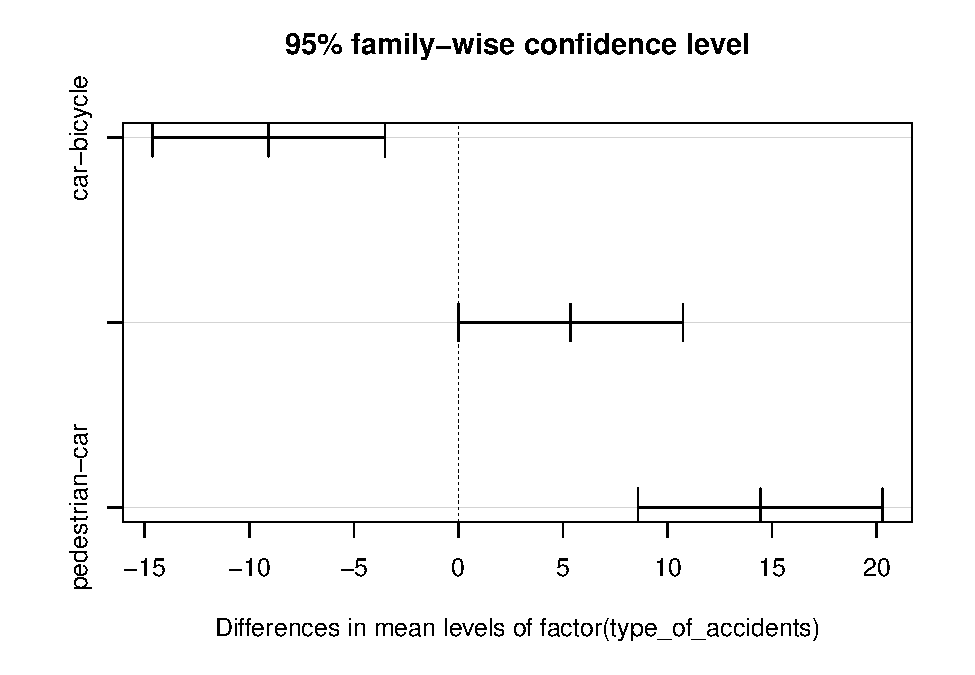
\includegraphics{HW4-tk2886-_files/figure-latex/unnamed-chunk-7-1.pdf}

Problem 3b:

\begin{Shaded}
\begin{Highlighting}[]
\NormalTok{test\_statistcs }\OtherTok{=}\NormalTok{ (}\DecValTok{15}\FloatTok{{-}17.67}\NormalTok{)}\SpecialCharTok{\^{}}\DecValTok{2}\SpecialCharTok{/}\FloatTok{17.67} \SpecialCharTok{+}\NormalTok{ (}\DecValTok{18}\FloatTok{{-}17.67}\NormalTok{)}\SpecialCharTok{\^{}}\DecValTok{2}\SpecialCharTok{/}\FloatTok{17.67} \SpecialCharTok{+}\NormalTok{ (}\DecValTok{20}\FloatTok{{-}17.67}\NormalTok{)}\SpecialCharTok{\^{}}\DecValTok{2}\SpecialCharTok{/}\FloatTok{17.67} \SpecialCharTok{+}\NormalTok{ (}\DecValTok{18}\FloatTok{{-}15.33}\NormalTok{)}\SpecialCharTok{\^{}}\DecValTok{2}\SpecialCharTok{/}\FloatTok{15.33} \SpecialCharTok{+}\NormalTok{ (}\DecValTok{15}\FloatTok{{-}15.33}\NormalTok{)}\SpecialCharTok{\^{}}\DecValTok{2}\SpecialCharTok{/}\FloatTok{15.33} \SpecialCharTok{+}\NormalTok{ (}\DecValTok{13}\FloatTok{{-}15.33}\NormalTok{)}\SpecialCharTok{\^{}}\DecValTok{2}\SpecialCharTok{/}\FloatTok{15.33}
\end{Highlighting}
\end{Shaded}

\begin{Shaded}
\begin{Highlighting}[]
\NormalTok{critical\_value }\OtherTok{=} \FunctionTok{qchisq}\NormalTok{(.}\DecValTok{95}\NormalTok{, }\DecValTok{1}\NormalTok{)}
\end{Highlighting}
\end{Shaded}

Problem 3c:

Ho: Relapse Status and types of anti-depressant are independent

Ha: Relase Status and types of anti-depressant are associated/dependent

\end{document}
